\documentclass[a4paper,10pt]{article}
\usepackage[utf8]{inputenc}
\usepackage{amsmath}
\usepackage{amsfonts}
\usepackage{amssymb}
\usepackage[german]{babel}
\setlength{\parindent}{0cm}
\usepackage{setspace}
\usepackage{mathpazo}
\usepackage{listings}
\usepackage{graphicx}
\usepackage{wasysym}
\usepackage{booktabs}
\usepackage{verbatim}
\usepackage{ulem}
\usepackage{enumerate}
\usepackage{hyperref}
\usepackage{ulem}
\usepackage{stmaryrd }
\usepackage[a4paper,
left=1.8cm, right=1.8cm,
top=2.0cm, bottom=2.0cm]{geometry}
\usepackage{tabularx}
\usepackage{tikz}
\usetikzlibrary{trees,petri,decorations,arrows,automata,shapes,shadows,positioning,plotmarks}

\lstdefinelanguage{clojure}%
{morekeywords={*,*1,*2,*3,*agent*,*allow-unresolved-vars*,*assert*,*clojure-version*,*command-line-args*,%
*compile-files*,*compile-path*,*e,*err*,*file*,*flush-on-newline*,*in*,*macro-meta*,%
*math-context*,*ns*,*out*,*print-dup*,*print-length*,*print-level*,*print-meta*,*print-readably*,%
*read-eval*,*source-path*,*use-context-classloader*,*warn-on-reflection*,+,-,->,->>,..,/,:else,%
<,<=,=,==,>,>=,@,accessor,aclone,add-classpath,add-watch,agent,agent-errors,aget,alength,alias,%
all-ns,alter,alter-meta!,alter-var-root,amap,ancestors,and,apply,areduce,array-map,aset,%
aset-boolean,aset-byte,aset-char,aset-double,aset-float,aset-int,aset-long,aset-short,assert,%
assoc,assoc!,assoc-in,associative?,atom,await,await-for,await1,bases,bean,bigdec,bigint,binding,%
bit-and,bit-and-not,bit-clear,bit-flip,bit-not,bit-or,bit-set,bit-shift-left,bit-shift-right,%
bit-test,bit-xor,boolean,boolean-array,booleans,bound-fn,bound-fn*,butlast,byte,byte-array,%
bytes,cast,char,char-array,char-escape-string,char-name-string,char?,chars,chunk,chunk-append,%
chunk-buffer,chunk-cons,chunk-first,chunk-next,chunk-rest,chunked-seq?,class,class?,%
clear-agent-errors,clojure-version,coll?,comment,commute,comp,comparator,compare,compare-and-set!,%
compile,complement,concat,cond,condp,conj,conj!,cons,constantly,construct-proxy,contains?,count,%
counted?,create-ns,create-struct,cycle,dec,decimal?,declare,def,definline,defmacro,defmethod,%
defmulti,defn,defn-,defonce,defprotocol,defstruct,deftype,delay,delay?,deliver,deref,derive,%
descendants,destructure,disj,disj!,dissoc,dissoc!,distinct,distinct?,do,do-template,doall,doc,%
dorun,doseq,dosync,dotimes,doto,double,double-array,doubles,drop,drop-last,drop-while,empty,empty?,%
ensure,enumeration-seq,eval,even?,every?,false,false?,ffirst,file-seq,filter,finally,find,find-doc,%
find-ns,find-var,first,float,float-array,float?,floats,flush,fn,fn?,fnext,for,force,format,future,%
future-call,future-cancel,future-cancelled?,future-done?,future?,gen-class,gen-interface,gensym,%
get,get-in,get-method,get-proxy-class,get-thread-bindings,get-validator,hash,hash-map,hash-set,%
identical?,identity,if,if-let,if-not,ifn?,import,in-ns,inc,init-proxy,instance?,int,int-array,%
integer?,interleave,intern,interpose,into,into-array,ints,io!,isa?,iterate,iterator-seq,juxt,%
key,keys,keyword,keyword?,last,lazy-cat,lazy-seq,let,letfn,line-seq,list,list*,list?,load,load-file,%
load-reader,load-string,loaded-libs,locking,long,long-array,longs,loop,macroexpand,macroexpand-1,%
make-array,make-hierarchy,map,map?,mapcat,max,max-key,memfn,memoize,merge,merge-with,meta,%
method-sig,methods,min,min-key,mod,monitor-enter,monitor-exit,name,namespace,neg?,new,newline,%
next,nfirst,nil,nil?,nnext,not,not-any?,not-empty,not-every?,not=,ns,ns-aliases,ns-imports,%
ns-interns,ns-map,ns-name,ns-publics,ns-refers,ns-resolve,ns-unalias,ns-unmap,nth,nthnext,num,%
number?,odd?,or,parents,partial,partition,pcalls,peek,persistent!,pmap,pop,pop!,pop-thread-bindings,%
pos?,pr,pr-str,prefer-method,prefers,primitives-classnames,print,print-ctor,print-doc,print-dup,%
print-method,print-namespace-doc,print-simple,print-special-doc,print-str,printf,println,println-str,%
prn,prn-str,promise,proxy,proxy-call-with-super,proxy-mappings,proxy-name,proxy-super,%
push-thread-bindings,pvalues,quot,rand,rand-int,range,ratio?,rational?,rationalize,re-find,%
re-groups,re-matcher,re-matches,re-pattern,re-seq,read,read-line,read-string,recur,reduce,ref,%
ref-history-count,ref-max-history,ref-min-history,ref-set,refer,refer-clojure,reify,%
release-pending-sends,rem,remove,remove-method,remove-ns,remove-watch,repeat,repeatedly,%
replace,replicate,require,reset!,reset-meta!,resolve,rest,resultset-seq,reverse,reversible?,%
rseq,rsubseq,second,select-keys,send,send-off,seq,seq?,seque,sequence,sequential?,set,set!,%
set-validator!,set?,short,short-array,shorts,shutdown-agents,slurp,some,sort,sort-by,sorted-map,%
sorted-map-by,sorted-set,sorted-set-by,sorted?,special-form-anchor,special-symbol?,split-at,%
split-with,str,stream?,string?,struct,struct-map,subs,subseq,subvec,supers,swap!,symbol,symbol?,%
sync,syntax-symbol-anchor,take,take-last,take-nth,take-while,test,the-ns,throw,time,to-array,%
to-array-2d,trampoline,transient,tree-seq,true,true?,try,type,unchecked-add,unchecked-dec,%
unchecked-divide,unchecked-inc,unchecked-multiply,unchecked-negate,unchecked-remainder,%
unchecked-subtract,underive,unquote,unquote-splicing,update-in,update-proxy,use,val,vals,%
var,var-get,var-set,var?,vary-meta,vec,vector,vector?,when,when-first,when-let,when-not,%
while,with-bindings,with-bindings*,with-in-str,with-loading-context,with-local-vars,%
with-meta,with-open,with-out-str,with-precision,xml-seq,zero?,zipmap
},%
   sensitive,% ???
   alsodigit=-,%
   morecomment=[l];,%
   morestring=[b]"%
  }[keywords,comments,strings]%

\lstset{language=Clojure,showstringspaces=false,
  basicstyle=\footnotesize\ttfamily,
  keywordstyle=\bfseries\color{green!40!black},
  commentstyle=\itshape\color{purple!40!black},
  identifierstyle=\color{blue},
  stringstyle=\color{orange}}

\newcommand{\rf}{\right\rfloor}
\newcommand{\lf}{\left\lfloor}
\newcommand{\tabspace}{15cm}
\newcommand{\N}{\mathbb{N}}
\newcommand{\Z}{\mathbb{Z}}

\begin{document}
\begin{center}
\Large{Grundlagen der künstlichen Intelligenz: Hausaufgabe 2} \\
\end{center}
\begin{tabbing}
Tom Nick \hspace{2cm}\= - 340528\\
Niklas Gebauer \> - 340942 \\
Leonard Witte \> - 341457 \\
Johannes Herrmann \> - xxxxxx\\
\end{tabbing}

\section*{Aufgabe 1}

Alle Aufgaben wurden in \textbf{Clojure1 1.5} geschrieben und benutzen nichts außer \textit{clojure.core} als namespace.
\subsubsection*{Backtracking}
\begin{lstlisting}
(def counter (atom 0))

(defn solve-stack [n]
  "exacly the algorithm mentioned in the exercise"
  (let [domains (vec (for [i (range n)] (vec (range n))))
        constrains [(fn [state] (= (count (distinct state)) (count state)))
                    (fn [state] (let [j (dec (count state))]
                                  (every? true? (for [i (range j)]
                                                  (not= (Math/abs (- i j))
                                                        (Math/abs (- ((domains i) (nth state (- j i)))
                                                                     ((domains j) (first state)))))))))]]
    (loop [[x & xs] [[]]]
      (if (or (nil? x) (= n (count x)))
        x
        (recur (concat (for [i (domains (count x))
                             :when (every? true? (map #(% (cons i x)) constrains))]
                         (do (swap! counter inc)
                             (cons i x))) xs))))))
\end{lstlisting}

\textbf{Erklärung:}
\begin{itemize}
  \item \textbf{domains} repräsentiert die Domain einer jeden Dame und sieht für \texttt{n = 2} so aus: \texttt{[[0, 1], [0, 1]]}.
  \item \textbf{constrains} ist eine Liste aus Funktionen die jeweils einen Belegungszustand bekommen, wobei eine Belegung eine Liste von 0 bis \texttt{n} Elementen ist, z.B. \texttt{[0, 1]}. Sie stellen die constrains dar. Eine Funktion testet das keine Dame eine andere horizontal schlagen kann und die andere, dass sie es nicht diagonal können. Die Funktionen liefern ein \texttt{Bool} zurück.
  \item \textbf{loop} dies ist die Rekursion und der eigentliche Algorhitmus. Zum Start bekommt die Funktion einen Stack mit einer leeren Belegung \texttt{[[]]}, durch destructuring setzen wird \texttt{x} \texttt{[]} zugewiesen. Als Rekursionsanker wird überprüft ob \texttt{x} einen Wert hat, also ob der Stack leer ist, oder ob wir eine gültige Belegung gefunden haben. In dieser Implementierung ist eine gültige Belegung eine Liste der Länge \texttt{n}. Falls eine der Bedingungen stimmt, wird die \texttt{x} zurückgegeben, also entweder eine gültige Belegung oder \texttt{nil} falls es keine Belegung gibt. Anonsten werden mittels list-comprehension die neuen Werte für den Stack bestimmt, wobei nur Werte auf den Stack gelegt werden die alle constrains beachten (backtracking). Der \texttt{counter} wird um für jeden expandierten Knoten um eins erhöht und zum Schluss werden die Werte vorne an den Stack gehängt.
\end{itemize}
\newpage
\subsubsection*{Backtracking + Forward Checking + Minimum Remaining Values}
\begin{lstlisting}
(def counter (atom 0))

(defn solve-stack-fc-mrv [n]
  "exacly the algorithm mentioned in the exercise with forward checking and mrv"
  (let [domains-initial (zipmap (range n) (repeat (range n)))
        constrains [(fn [[x1 y1] [x2 y2]] (not= y1 y2))
                    (fn [[x1 y1] [x2 y2]]
                      (not= (Math/abs (- x1 x2))
                            (Math/abs (- y1 y2))))]
        forward-check (fn [x1 y1 domains]
                        (apply merge
                               (for [[x2 domain] domains]
                                 {x2 (filter (fn [y2] (every? true? (map #(% [x1 y1] [x2 y2]) constrains))) domain)})))]
    (loop [[[state domains] & xs] [[{} domains-initial]]]
      (if (or (nil? state) (= n (count state)))
        (map second (sort state))
        (let [[x domain] (rand-nth ((comp second first) (sort (group-by (comp count second) domains))))
              domains (dissoc domains x)
              states (filter #(every? (comp (partial < 0) count) (second %))
                             (for [y domain]
                               [(assoc state x y) (forward-check x y domains)]))]
          (recur (do (swap! counter (partial + (count states)))
                     (concat states xs))))))))
\end{lstlisting}
\textbf{Erklärung}
\begin{itemize}
  \item \textbf{domains-initial} repräsentiert die initiellen Domains einer jeden Dame und sieht für \texttt{n = 2} so aus: \texttt{\{0: [0 1], 1: [0 1]\}}. Also dictionary/map wo die keys die jeweilige Dame sind und die values die Domain der Dame.
    \item \textbf{constrains} ist eine Liste aus Funktionen die jeweils einen 2 x/y Koordinaten bekommen, jede Koordinate ist die Position einer Dame. Sie überprüfen ob die Damen sich horizontal oder diagonal schlagen können.
    \item \textbf{forward-check} Dies ist der forward-check, die Funktion bekommt die Position der zu setzenden Dame \texttt{x1 y1} und die aktuellen Domains \texttt{domains}, wobei die Domain der zu setzenden Dame entfernt wurde. Sie liefert die \textit{bereinigten} Domains zurück.
    \item \textbf{loop} Jeder \textit{Node} wird mittels eines Vektors aus Belegung und Domains dargestellt, der Start-stack besteht damit aus einem \textit{Node} der wiederum aus einer leeren Belegung hat und den initiellen Domains besteht: \texttt{[{} domains-initial]}. Der Rekursionsanker ist ähnlich wie zuvor. Wenn die Funktion nicht terminiert bestimmt sie nach \textbf{mrv-Prinzip} den nächsten Wert \texttt{(rand-nth ...)}. Die Domain für diesen Wert wird entfernt (siehe forward-check), mittels list-comprehension werden alle gültigen nächsten Zustände ermittelt, bei welchen der Forward-check die Domains eingeschränkt hat. Falls es keine gültigen Folgezustände für die aktuelle Belegung gibt, ist \textbf{states} leer, und im nächsten Rekursionschritt wird der eine andere Belegung getestet: \texttt{(recur (concat states xs))}. \texttt{(swap!..)} ist dafür da den Counter hochzuzählen.
\end{itemize}
\newpage
\subsubsection*{Backtracking + Arc Consistency + Minimum Remaining Values}
\begin{lstlisting}
(defn solve-stack-arc-mrv [n]
  "exacly the algorithm mentioned in the exercise with arc-consistency and mrv"
  (let [domains-initial (zipmap (range n) (repeat (range n)))
        constrains [(fn [[x1 y1] [x2 y2]] (not= y1 y2))
                    (fn [[x1 y1] [x2 y2]]
                      (not= (Math/abs (- x1 x2))
                            (Math/abs (- y1 y2))))]
        arc-consistency (fn [domains]
                          (let [arcs
                                (for [[x1 d1] domains
                                      [x2 d2] domains
                                      :when (not= x1 x2)]
                                  [x1 x2])]
                            (loop [[[x1 x2] & xs] arcs domains domains]
                              (if (nil? x1)
                                domains
                                (let [d1 (domains x1)
                                      d2 (domains x2)
                                      d1-new (for [y1 d1
                                                   :when (not (empty? (filter (fn [y2]
                                                                   (every? true? (map #(% [x1 y1]
                                                                                          [x2 y2])
                                                                                      constrains))) d2)))] y1)
                                      new-arcs (for [[x3 y3] domains
                                                     :when (and (not= x3 x2) (not= x3 x1))] [x3 x1])]
                                  (if (not= (sort d1-new) (sort d1))
                                    (recur (concat xs new-arcs) (assoc domains x1 d1-new))
                                    (recur xs domains)))))))]
    (loop [[[state domains] & xs] [[{} domains-initial]]]
      (if (or (nil? state) (= n (count state)))
        (map second (sort state))
        (let [[x domain] (rand-nth ((comp second first)
                                    (sort (group-by (comp count second)
                                                    (filter (fn [[x d]] (not (state x))) domains)))))
              states (for [y domain
                           :let [domains-new (arc-consistency (assoc domains x [y]))]
                           :when (empty? (filter (fn [[x d]] (zero? (count d))) domains-new))]
                       [(assoc state x y) domains-new])
              states states]
          (recur (do (swap! counter (partial + (count states)))
                     (concat states xs))))))))
\end{lstlisting}
\textbf{Erklärung}
\begin{itemize}
  \item \textbf{domains-initial und constrains} Genau wie in forward-check.
    \item \textbf{arc-conistency} Bekommt als Eingabe alle Domains, wobei die Domains von gesetzten Damen einstellig sind.
    \item \textbf{loop} Ziemlich genau wie beim forward-check, nur entfernen wir nicht die belegten Variablen aus \texttt{domains} da wir die Belegung für den arc-consistency check brauchen. Dadurch hat sich aber etwas die Berechnung für die nächste Varibale geändert (nur Variablen aus \texttt{domains} deren key noch nicht in \texttt{state} ist): \texttt{(filter (fn [[x d]] (not (state x))) domains)}. Für den aktuellen Zustand werden dann wieder die Folgezustände asugerechnet, wobei keiner eine leere domain haben darf: \texttt{:when (empty? (filter (fn [[x d]] (zero? (count d))) domains-new))}.
\end{itemize}
\newpage
\subsection*{Diagramme}
Alle Grafiken wurden mit nvd3.js + d3.js erstellt und die interaktiven Versionen davon sind in charts.html zu finden. Die Rohdaten sind in \texttt{results.json}. \texttt{queens\$solve\_stack\_fc\_mrv@1c0b5c67} steht für \textbf{BT + FC + MRV}, \texttt{queens\$solve\_stack\_arc\_mrv@75e08420} steht für \textbf{BT + ARC + MRV} und \texttt{queens\$solve\_stack@3e55747} steht für \textbf{BT}.
\begin{center}
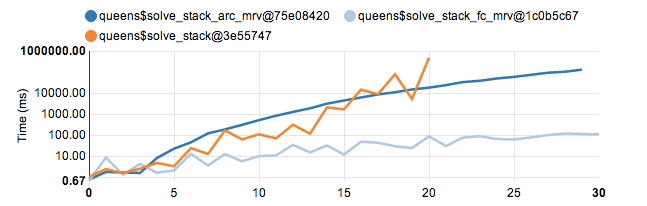
\includegraphics[scale=0.7]{chart_one.png} \\
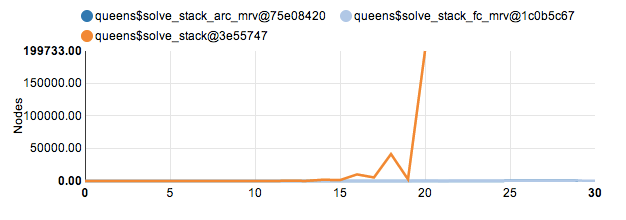
\includegraphics[scale=0.7]{chart_two.png} \\
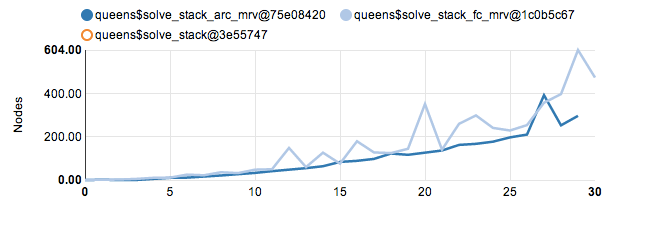
\includegraphics[scale=0.7]{chart_three.png} \\
\end{center}

\section*{Aufgabe 2}
\begin{enumerate}[~~a)]

\item
Das Zuordnungsproblem in 2-konsistentem Zustand: \\
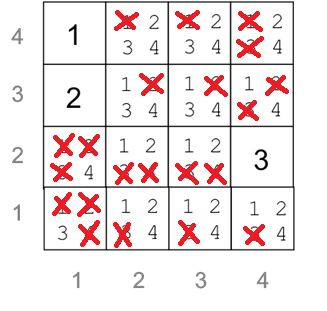
\includegraphics[scale=0.7]{Aufgabe2a}

\item
Wir wählen für den nächsten Schritt die MRV-Heuristik, da wir Variablen mit einem kleinen Wertebereich möglichst schnell belegen wollen, um früh auf mögliche Fehler zu stoßen. Allerdings ergibt es nach dem Herstellen des 2-konsistenten Zustands keinen Sinn, Variablen auszuwählen, die einen ein-elementigen Wertebereich haben, denn aufgrund der 2-Konsistenz kann keine zukünftige Belegung anderer Variablen dazu führen, dass die Ein-elementigen nicht mehr belegt werden könnten. Daher können sie später belegt werden, wenn der Rest des Zuordnungsproblems gelöst ist. \\
Da wir im nächsten Schritt Forward Checking verwenden werden, ist es sinnvoll MCV als Tie-Breaker zu verwenden, um eine Variable zu wählen, die den Wertebereich von möglichst vielen anderen Variablen betrifft, falls es mehrere Variablen gibt, nachdem die MRV-Heuristik angewendet wurde.\\
Für unser Problem sind die Wertebereiche der Variablen $(2,2), (3,2), (4,3),$ und $(4.4)$ im 2-konsistenten Zustand alle gleich klein (zwei Elemente). \\
Der Tie-Breaker MCV liefert uns nun $(2,2)$ und $(3,2)$ da diese jeweils Constraints zu noch 5 unbelegt Variablen haben (die anderen beiden kandidaten jeweils nur 4). Wir wählen eine dieser Variablen zufällig für unseren nächsten Schritt.\\
\item
Sei die von uns zufällig gewählte Variable der beiden oben genannten Kandidaten $(2,2)$. Dann belegen wir diese mit dem Wert $1$ und erhalten so mittels Forward-Checking folgende eingeschränkte Wertebereiche: \\
$(2,1) = \{2,4\} \\
(2,3) = \{ 3,4\} \\
(3,2) = \{2\}$\\
Alle anderen Wertebereiche bleiben unverändert.
\end{enumerate}

\section*{Aufgabe 3}

\begin{enumerate}[~~a)]

\item
Anzahl der Konflikte zu Beginn (alle Knoten weiss): 10 \\
\\
\begin{tabular}{|c|c|c|c|}
\hline
Schritt & Knoten & Farbe & resultierende Konflikte  \\ \hline
1. & B & Grau & 6 \\ \hline
2. & A & Schwarz & 4 \\ \hline
3. & C & Schwarz & 2 \\ \hline
4. & F & Grau & 1 \\ \hline
\end{tabular} \\ \\
Ergebnis: Der Algorithmus terminiert, ohne eine Lösung (vollständige und konsistente Belegung) zu finden.

\item
Wir ändern die Tie-Break-Regel nun so, dass wir den lexikographisch größten Knoten wählen, wenn die Anzahl der resultierenden Konflikte gleich ist. Somit würde der Algorithmus wie folgt ablaufen: \\
\\
\begin{tabular}{|c|c|c|c|}
\hline
Schritt & Knoten & Farbe & resultierende Konflikte  \\ \hline
1. & B & Grau & 6 \\ \hline
2. & G & Grau & 4 \\ \hline
3. & E & Schwarz & 2 \\ \hline
4. & A & Schwarz & 0 \\ \hline
\end{tabular} \\ \\
Ergebnis: Wir finden eine Lösung für das CSP!

\end{enumerate}

\section*{Aufgabe 4}

\section*{Aufgabe 5}
\begin{enumerate}[~~a)]

\item Spielbaum mit allen Minimax-Werten an den Knoten: \\
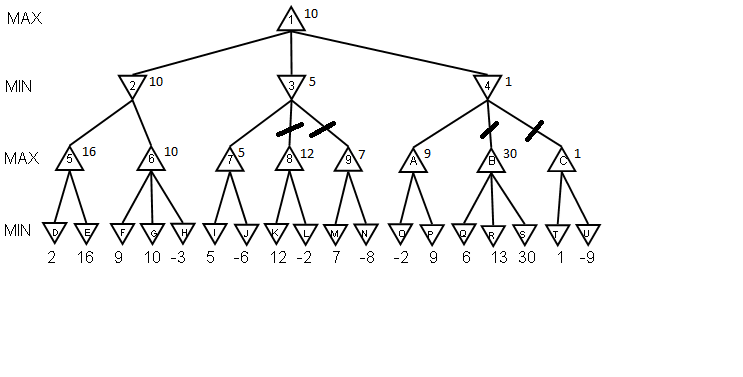
\includegraphics[scale=1]{Aufgabe5}

\item Die Zweige, die durch Cut-Offs entfernt würden, sind im obigen Bild markiert.

\end{enumerate}

\end{document}
